\chapter{Implementierung}\label{implementierung}

Dieses Kapitel dokumentiert die konkrete Umsetzung des in Kapitel~\ref{systemkonzeption} konzipierten Systems. Es gliedert sich in Backend-Implementierung (Abschnitt~\ref{backend-implementierung}), KI-Generierungspipeline (Abschnitt~\ref{ki-generierungspipeline}), Frontend (Abschnitt~\ref{frontend-implementierung}), n8n-Workflows (Abschnitt~\ref{n8n-workflow-implementierung}), Qualitätssicherung und Tests (Abschnitt~\ref{qualitätssicherung-und-tests}) sowie Deployment (Abschnitt~\ref{deployment}).


\section{Backend-Implementierung}\label{backend-implementierung}

Das Backend setzt die in Abschnitt~\ref{backend-konzeption} konzipierten Schichten als lauffähige FastAPI-Anwendung um. Es gliedert sich in Projektstruktur und Application Entry Point (Abschnitt~\ref{projektstruktur-und-application-entry-point}), Datenmodelle und API-Validierung (Abschnitt~\ref{datenmodelle-datenbankschema-und-api-validierung}), API-Router und Endpunktstruktur (Abschnitt~\ref{api-router-endpunktstruktur}), Ticker-Service und Domänenlogik (Abschnitt~\ref{ticker-service-domuxe4nenlogik}) sowie LLM-Service und Provider-Dispatch (Abschnitt~\ref{llm-service-prompt-aufbau-und-provider-dispatch}).

\subsection{Projektstruktur und Application Entry
Point}\label{projektstruktur-und-application-entry-point}

Das Backend gliedert sich unter \texttt{backend/app/} in sieben funktionale Pakete:

\begin{verbatim}
backend/app/
|-- api/v1/          # HTTP-Router (FastAPI)
|-- models/          # SQLAlchemy ORM-Modelle (17 Dateien)
|-- repositories/    # Datenbankzugriff (je Entitaet eine Klasse)
|-- schemas/         # Pydantic-Schemas (Request / Response)
|-- services/        # Fachliche Services (llm_service, ticker_service)
|-- utils/           # Hilfsmodule (context_builders, metrics)
`-- core/            # Konfiguration, Datenbankverbindung, Enums, Konstanten
\end{verbatim}

Diese Aufteilung setzt das in Abschnitt~\ref{interne-schichtstruktur} konzipierte Repository-Service-Router-Muster um.

\begin{figure}[H]
\centering
\DiagramBackendSchichten
\caption{Backend-Schichtenarchitektur: Router \textrightarrow{} Service \textrightarrow{} Repository \textrightarrow{} DB}
\label{fig:backend-schichten}
\end{figure}

\texttt{app/main.py} ist der einzige Einstiegspunkt. Er umfasst zwölf Router-Registrierungen: elf Router unter \texttt{/api/v1} sowie den WebSocket-Router \texttt{/ws/media}. Da der Ticker-Bereich intern auf drei Dateien aufgeteilt ist (vgl. Abschnitt~\ref{api-router-endpunktstruktur}), ergeben sich 13 Router-Dateien in \texttt{api/v1/}. Darüber hinaus konfiguriert \texttt{app/main.py} CORS-Middleware und bindet statische Dateien (Thumbnail-Cache) ein. Beim Start führt ein \texttt{lifespan}-Context-Manager \texttt{alembic upgrade head} aus, sodass ausstehende Migrationen automatisch eingespielt werden, bevor der erste Request eintrifft. Die Datenbankverbindung wird per FastAPI Dependency Injection in jeden Router injiziert. \texttt{core/database.py} stellt einen \texttt{get\_db()}-Generator bereit, der pro Anfrage eine Session öffnet und am Anfrageende garantiert schließt.


\subsection{Datenmodelle: Datenbankschema und
API-Validierung}\label{datenmodelle-datenbankschema-und-api-validierung}

Das Schema umfasst 17 ORM-Modelle (18 Datenbanktabellen). Die
zentralen Domänenobjekte sind:

{\small\def\LTcaptype{none} % do not increment counter
\begin{longtable}[]{@{}
  >{\raggedright\arraybackslash}p{(\linewidth - 4\tabcolsep) * \real{0.2300}}
  >{\raggedright\arraybackslash}p{(\linewidth - 4\tabcolsep) * \real{0.2700}}
  >{\raggedright\arraybackslash}p{(\linewidth - 4\tabcolsep) * \real{0.5000}}@{}}
\toprule\noalign{}
\begin{minipage}[b]{\linewidth}\raggedright
Modell
\end{minipage} & \begin{minipage}[b]{\linewidth}\raggedright
Tabelle
\end{minipage} & \begin{minipage}[b]{\linewidth}\raggedright
Kernfelder
\end{minipage} \\
\midrule\noalign{}
\endhead
\bottomrule\noalign{}
\endlastfoot
\texttt{Match} & \texttt{matches} & \texttt{id}, \texttt{uid},
\texttt{match\_state}, \texttt{match\_phase}, \texttt{ticker\_mode} \\
\texttt{Event} & \texttt{events} & \texttt{id}, \texttt{match\_id},
\texttt{event\_type}, \texttt{time}, \texttt{description} \\
\texttt{SyntheticEvent} & \texttt{synthetic\_events} & \texttt{id},
\texttt{match\_id}, \texttt{type}, \texttt{data} (JSONB) \\
\texttt{TickerEntry} & \texttt{ticker\_entries} & → siehe unten \\
\texttt{StyleReference} & \texttt{style\_references} &
\texttt{event\_type}, \texttt{instance}, \texttt{league}, \texttt{text}
(Few-Shot) \\
\end{longtable}
}

Weitere Stammdaten-Modelle (Country, Team, Competition, Lineup, MatchStatistic, PlayerStatistic, MediaQueue, MediaClip) folgen dem gleichen Grundmuster und sind vollständig in \texttt{app/models/} implementiert. Die 18. Datenbanktabelle (\texttt{settings}) wird direkt per Alembic-Migration als Key-Value-Store angelegt und hat kein ORM-Modell.

Das \texttt{TickerEntry}-Modell ist zentral für den Lifecycle des Systems: Es verknüpft über \texttt{event\_id} (FK auf \texttt{events})
und \texttt{synthetic\_event\_id} (FK auf \texttt{synthetic\_events})
den generierten Text mit seinem Auslöser. Die Felder \texttt{status}
(\texttt{draft}/\allowbreak\texttt{published}/\allowbreak\texttt{rejected}/\allowbreak\texttt{deleted}) und
\texttt{source} (\texttt{ai}/\texttt{manual}) bilden den
Ticker-Lifecycle ab (vgl. Abschnitt~\ref{status-lifecycle-und-betriebsmodi}). Drei zusammengesetzte Indizes
(\texttt{ix\_ticker\_match\_status}, \texttt{ix\_ticker\_match\_phase},
\texttt{ix\_ticker\_event\_id}) optimieren die häufigsten Abfragen:
publizierte Einträge je Spiel, Phase-Filter und den
Deduplizierungs-Check per Event. Beide Enums (\texttt{status} und \texttt{source}) werden als nicht-nativ gespeichert (\texttt{native\_enum=False}), damit Migrationen ohne PostgreSQL-seitige Enum-Typ-Änderungen auskommen, da solche Änderungen sonst eine exklusive Tabellensperre erfordern würden.

Das JSONB-Feld \texttt{synthetic\_events.data} speichert kontextabhängig strukturierte Ereignisdaten, deren Schema je nach \texttt{type} variiert. Beispiel für den Typ \texttt{pre\_match\_h2h}:

\begin{Shaded}
\begin{Highlighting}[]
\NormalTok{\{}
  \StringTok{"fixture\_id"}\NormalTok{: 1035443,}
  \StringTok{"matches"}\NormalTok{: [\{}
    \StringTok{"date"}\NormalTok{: }\StringTok{"2024-10-05"}\NormalTok{,}
    \StringTok{"home\_team"}\NormalTok{: }\StringTok{"Eintracht Frankfurt"}\NormalTok{,}
    \StringTok{"away\_team"}\NormalTok{: }\StringTok{"FC Bayern München"}\NormalTok{,}
    \StringTok{"goals\_home"}\NormalTok{: 2, }\StringTok{"goals\_away"}\NormalTok{: 1,}
    \StringTok{"winner"}\NormalTok{: }\StringTok{"Eintracht Frankfurt"}
  \NormalTok{\}, ...]}
\NormalTok{\}}
\end{Highlighting}
\end{Shaded}

Für jeden Router gibt es eigenständige Pydantic-Schemas für Create-, Update- und Response-Strukturen. Die Stammdaten-Schemas (Match, Event, Team, Competition u.\,a.) nutzen \texttt{alias\_generator=to\_camel} für konsistente camelCase-API-Verträge bei Python-internem snake\_case. Ticker- und Medien-Schemas serialisieren Felder direkt ohne Alias-Konvertierung.

Jede Entität hat ein dediziertes Repository, das alle SQL-Operationen
kapselt. Alle Repositories erben von
\texttt{BaseRepository{[}T{]}}, die \texttt{exists()} generisch
bereitstellt. Jede Instanz erhält eine \texttt{Session} im Konstruktor.
Das \texttt{MatchRepository} lädt Heim- und Auswärtsteam, Wettbewerb und
Saison per \texttt{joinedload} in einer einzigen Abfrage vor, da die
KI-Generierungsroute vollständige Kontext-Daten benötigt.

\subsection{API-Router:
Endpunktstruktur}\label{api-router-endpunktstruktur}

Der Ticker-Bereich ist in drei Router aufgeteilt, die gemeinsam unter
\texttt{/api/v1/ticker} eingehängt werden:

{\def\LTcaptype{none} % do not increment counter
\begin{longtable}[]{@{}
  >{\raggedright\arraybackslash}p{(\linewidth - 4\tabcolsep) * \real{0.2500}}
  >{\raggedright\arraybackslash}p{(\linewidth - 4\tabcolsep) * \real{0.3000}}
  >{\raggedright\arraybackslash}p{(\linewidth - 4\tabcolsep) * \real{0.4500}}@{}}
\toprule\noalign{}
\begin{minipage}[b]{\linewidth}\raggedright
Router
\end{minipage} & \begin{minipage}[b]{\linewidth}\raggedright
Datei
\end{minipage} & \begin{minipage}[b]{\linewidth}\raggedright
Kernoperationen
\end{minipage} \\
\midrule\noalign{}
\endhead
\bottomrule\noalign{}
\endlastfoot
\texttt{ticker\_crud} & \texttt{ticker\_crud.py} & GET list, GET single,
PATCH status, DELETE, POST manual \\
\texttt{ticker\_generate} & \texttt{ticker\_generate.py} & POST
generate/\{event\_id\}, generate-synthetic, generate-synthetic-batch, generate-match-phases \\
\texttt{ticker\_batch} & \texttt{ticker\_batch.py} & POST
generate-bulk, translate-batch \\
\end{longtable}
}

Der Batch-Endpunkt
\texttt{POST\ /api/v1/ticker/translate-batch/\{match\_id\}} ruft für
alle Einträge eines Spiels mit vorhandenem Text (publizierte und Entwürfe) den LLM-Service mit
reduzierter Temperatur (\texttt{0.1}) auf, um sprachlich
deterministische Übersetzungen zu erzeugen, eine gegenüber der
Originalgenerierung abweichende Parametrisierung.

Die fünf kritischen Lifecycle-Endpunkte sind:

{\def\LTcaptype{none}
\begin{longtable}[]{@{}
  >{\raggedright\arraybackslash}p{(\linewidth - 4\tabcolsep) * \real{0.48}}
  >{\raggedright\arraybackslash}p{(\linewidth - 4\tabcolsep) * \real{0.52}}@{}}
\toprule\noalign{}
Endpunkt & Funktion \\
\midrule\noalign{}
\endhead
\bottomrule\noalign{}
\endlastfoot
{\small\texttt{POST /api/v1/events}} & Erstellt oder aktualisiert ein Spielereignis per Upsert (nach \texttt{sourceId}); n8n Workflow~09 schreibt Ereignisse alternativ direkt per SQL \\
{\small\texttt{POST /api/v1/ticker/generate/\{event\_id\}}} & Generiert einen KI-Ticker-Eintrag für ein konkretes Ereignis; wird von n8n Workflow~09 nach dem Ereignis-Import aufgerufen \\
{\small\texttt{PATCH /api/v1/ticker/\{id\}}} & Generisches Update (Text, Status, Stil); dedizierte Shortcuts \texttt{/publish}, \texttt{/reject} für Coop-Flow \\
{\small\texttt{POST /api/v1/ticker/manual}} & Erstellt einen manuellen Eintrag ohne LLM-Aufruf \\
{\small\texttt{PATCH /api/v1/matches/\{matchId\}}} & Aktualisiert Spielzustand (\texttt{match\_state}) und Phase (\texttt{match\_phase}); Phasenübergänge steuert n8n Workflow~14 zusätzlich per direktem SQL \\
\end{longtable}
}

Die API umfasst insgesamt 71 Routen (27 GET, 22 POST, 9 DELETE, 8 PATCH, 5 PUT) in vier funktionalen Bereichen: Stammdaten, Ticker-Lifecycle, Medien/Clips und Spielkontext. Die vollständige Endpunktliste ist über die automatisch generierte OpenAPI-Dokumentation unter \texttt{/api/docs} erreichbar.

Neben den HTTP-Routen registriert \texttt{main.py} den WebSocket-Router \texttt{/ws/media}. Dessen \texttt{MediaConnectionManager} hält eine In-Memory-Liste aktiver WebSocket-Verbindungen und stellt eine \texttt{broadcast()}-Methode bereit, die eingehende Medien-Payloads als JSON an alle verbundenen Redakteur-Clients sendet. Tote Verbindungen werden beim nächsten Broadcast-Versuch automatisch entfernt. Der Auslöser ist \texttt{POST /api/v1/media/incoming}: Sobald n8n WF08 eine ScorePlay-Asset-URL übermittelt, speichert dieser Endpunkt die URL in \texttt{media\_queue} und ruft \texttt{manager.broadcast()} auf, sodass das Frontend-Media-Panel den Treffer ohne Polling in Echtzeit empfängt.


\subsection{Ticker-Service:
Domänenlogik}\label{ticker-service-domuxe4nenlogik}

Der \texttt{ticker\_service} kapselt die Domänenlogik für KI-Einträge.
Er koordiniert Datenbankabfragen, Kontextaufbau und den LLM-Aufruf, hält
aber die Schichten klar getrennt: \texttt{llm\_service.py} hat
keine Datenbankabhängigkeit.

Der Service umfasst vier zentrale Funktionen. \texttt{score\_at\_event()}
berechnet den Spielstand zum Zeitpunkt eines Torereignisses: Da die
Football-API den kumulativen Stand liefert, muss der Stand \emph{vor}
dem aktuellen Event rekonstruiert werden. Eigentore werden korrekt
verarbeitet, da API-Football \texttt{team\_id} stets auf den
Nutznießer des Tores setzt (auch bei Eigentoren). \texttt{build\_match\_context()} erstellt das
Kontext-Dictionary für den LLM-Prompt aus Teamnamen, aktuellem Stand,
Matchzustand, Spielminute und Liga.

Die Kontextanreicherung (Stufe~2 der Pipeline) verläuft je nach Ereignistyp unterschiedlich. Für Live-Events (\texttt{goal}, \texttt{card} u.\,a.) erzeugt \texttt{build\_context\_data()} ein Dict aus Teamnamen und Spielstand, das \texttt{build\_context\_str()} anschließend als \texttt{ctx\_match\_info}-Block in den Prompt einbettet. Für synthetische Pre-Match-Events (z.\,B. \texttt{pre\_match\_h2h}) liefert \texttt{synthetic.data} die JSONB-Nutzdaten direkt — also exakt die Daten, die WF07 zuvor aus der Football-API importiert und in \texttt{synthetic\_events} persistiert hat. \texttt{build\_context\_str()} wählt anhand des \texttt{event\_type} den passenden Formatter (\texttt{ctx\_h2h}, \texttt{ctx\_injuries}, \texttt{ctx\_standings} u.\,a.) und übersetzt die strukturierten JSON-Daten in lesbare Prompt-Zeilen.

\texttt{call\_llm()} ist der zentrale, Semaphore-gesicherte LLM-Aufruf.
Er lädt zunächst aus dem \texttt{StyleReferenceRepository} bis zu drei
Stilbeispiele für \texttt{event\_type\ +\ instance\ +\ league} als
Few-Shot-Kontext und delegiert dann an \texttt{generate\_ticker\_text()}:

\begin{Shaded}
\begin{Highlighting}[]
\ControlFlowTok{async} \ControlFlowTok{with}\NormalTok{ \_llm\_semaphore:   }\CommentTok{\# asyncio.Semaphore(settings.LLM\_CONCURRENCY)}
    \ControlFlowTok{return} \ControlFlowTok{await}\NormalTok{ generate\_ticker\_text(}
\NormalTok{        event\_type}\OperatorTok{=}\NormalTok{event\_type,}
\NormalTok{        style\_references}\OperatorTok{=}\NormalTok{style\_references,  }\CommentTok{\# aus DB geladen}
\NormalTok{        ...}
\NormalTok{    )}
\end{Highlighting}
\end{Shaded}

Die Semaphore ist auf Modulebene als Singleton definiert
(\texttt{\_llm\_semaphore\ =\ asyncio.Semaphore(settings.LLM\_CONCURRENCY)},
Standard: 8) und begrenzt gleichzeitige LLM-Aufrufe pro FastAPI-Prozessinstanz. Bei einem Multi-Worker-Deployment (z.\,B. Gunicorn mit $n$ Workern) verfügt jeder Worker über eine eigene Semaphore, sodass systemweit bis zu $n \times 8$ parallele LLM-Aufrufe möglich wären. Für prozessübergreifende Limits wäre eine externe Rate-Limiting-Schicht erforderlich (vgl. Abschnitt~\ref{technische-einordnung}).

\texttt{make\_ai\_entry()} schließlich ist ein schlanker Builder, der aus
den LLM-Ergebnissen ein \texttt{TickerEntryCreate}-Schema erzeugt,
\texttt{source="ai"} setzt und den initialen Status abhängig vom
Aufrufkontext festlegt (\texttt{draft} im Co-op-Modus,
\texttt{published} im Auto-Modus).


\subsection{LLM-Service: Prompt-Aufbau und
Provider-Dispatch}\label{llm-service-prompt-aufbau-und-provider-dispatch}

Der \texttt{ticker\_service} delegiert die eigentliche Textgenerierung an den \texttt{LLMService}. Dieser instanziiert beim Start den passenden Client und ruft ihn über ein Dispatch-Dictionary auf:

\begin{Shaded}
\begin{Highlighting}[]
\NormalTok{dispatch }\OperatorTok{=}\NormalTok{ \{}
    \StringTok{"mock"}\NormalTok{:       }\VariableTok{self}\NormalTok{.\_generate\_mock\_text,}
    \StringTok{"gemini"}\NormalTok{:     }\VariableTok{self}\NormalTok{.\_generate\_gemini\_text,}
    \StringTok{"openrouter"}\NormalTok{: }\VariableTok{self}\NormalTok{.\_generate\_openrouter\_text,}
    \StringTok{"openai"}\NormalTok{:     }\VariableTok{self}\NormalTok{.\_generate\_openai\_text,}
    \StringTok{"anthropic"}\NormalTok{:  }\VariableTok{self}\NormalTok{.\_generate\_anthropic\_text,}
\NormalTok{\}}
\ControlFlowTok{return}\NormalTok{ dispatch[}\VariableTok{self}\NormalTok{.provider](}\OperatorTok{**}\NormalTok{kwargs)}
\end{Highlighting}
\end{Shaded}

Die Auswahl des aktiven Providers erfolgt zur Startzeit durch \texttt{\_build\_singleton()}, das das Dictionary \texttt{\_PROVIDER\_KEY\_MAP} (vgl. Abschnitt~\ref{multi-provider-architektur}) iteriert und den ersten Eintrag mit gesetztem API-Key aktiviert. Die Insertion-Order bestimmt die Priorität in der Konfigurationskette.

Vorab normalisiert eine \texttt{EVENT\_TYPE\_MAP} externe API-Strings auf einheitliche interne Bezeichner (\texttt{goal}, \texttt{card} etc.). Unbekannte Typen fallen auf \texttt{"comment"} zurück. Der Prompt wird über vier modulare Hilfsmethoden (\texttt{\_build\_event\_lines}, \texttt{\_build\_context\_str}, \texttt{\_build\_few\_shot\_block}, \texttt{\_build\_prematch\_parts}) zusammengesetzt, die fehlende Parameter auslassen, statt den Prompt zu invalidieren. Der Regelblock (\texttt{\#\#\# REGELN}) ist direkt in \texttt{\_build\_prompt} eingebettet (vgl. Abschnitt~\ref{prompt-engineering-strategie}).

Als Standardmodell im Deployment wird \texttt{google/gemini-2.0-flash-lite-001} über OpenRouter eingesetzt (vgl. Abschnitt~\ref{multi-provider-architektur} für die Begründung der Modellwahl). Die folgende Tabelle zeigt alle Provider der Prioritätskette mit ihren Standardmodellen. Temperatur für Textgenerierung ist einheitlich \texttt{LLM\_TEMPERATURE = 0.5}, für Übersetzungen \texttt{LLM\_TRANSLATION\_TEMPERATURE = 0.1}.

{\def\LTcaptype{none}
\begin{longtable}[]{@{}llll@{}}
\toprule\noalign{}
Priorität & Provider & Standard-Modell & Fallback \\
\midrule\noalign{}
\endhead
\bottomrule\noalign{}
\endlastfoot
1 & OpenRouter & \texttt{google/gemini-2.0-flash-lite-001} & --- \\
2 & Gemini    & \texttt{gemini-2.0-flash-lite-001}         & --- \\
3 & OpenAI    & \texttt{gpt-4o-mini}                       & --- \\
4 & Anthropic & \texttt{claude-haiku-4-5-20251001}         & --- \\
5 & Mock      & regelbasierte Templates                    & immer verfügbar \\
\end{longtable}
}

Als LLM-Parameter werden \texttt{temperature=0.5} für stilistische Variation und \texttt{max\_tokens} aus \texttt{LLM\_MAX\_TOKENS} gesetzt. Alle Prompts werden als einzelne User-Nachricht übermittelt. Der Rollenkontext ist direkt in den Prompttext eingebettet (vgl. Abschnitt~\ref{prompt-engineering-strategie}). Der \texttt{language}-Parameter für die Zielsprache wird ebenfalls direkt in den Prompt eingebettet und ermöglicht native Generierung in Deutsch, Englisch, Spanisch oder Französisch ohne sprachspezifische Prompt-Varianten (vgl. Abschnitt~\ref{mehrsprachige-textgenerierung-konzept}).

Für die Fehlerbehandlung unterscheidet der Service zwei Backoff-Strategien: Bei Rate-Limit-Fehlern (HTTP~429) greift lineares Backoff (\texttt{30\,s / 60\,s}), bei transienten Fehlern exponentielles Backoff (\texttt{1\,s / 2\,s}), jeweils bis zu \texttt{LLM\_RETRY\_ATTEMPTS} (3) Wiederholungen. Danach wird die ursprüngliche Ausnahme weitergereicht.


\section{KI-Generierungspipeline}\label{ki-generierungspipeline}

Die fünfstufige LLM-Pipeline verarbeitet eingehende Events vom Datenimport bis zum gespeicherten Ticker-Eintrag. Die Stufen Kontextanreicherung, Prompt-Aufbau und LLM-Aufruf sind in Abschnitt~\ref{backend-implementierung} dokumentiert. Dieser Abschnitt beschreibt die übergreifende Pipeline-Mechanik und Idempotenz (Abschnitt~\ref{pipeline-mechanik-und-idempotenz}) sowie Betriebsmodi und Statusübergänge (Abschnitt~\ref{betriebsmodi-und-statusuxfcberguxe4nge}).

\subsection{Pipeline-Mechanik und Idempotenz}\label{pipeline-mechanik-und-idempotenz}

Die Pipeline durchläuft fünf Stufen: Event-Import, Kontextanreicherung, Prompt-Aufbau, LLM-Aufruf und Persistenz. Abbildung~\ref{fig:event-workflow} zeigt die Stufenabfolge im Überblick. Abbildung~\ref{fig:ki-generierungspipeline} stellt den vollständigen Ablauf vom Ereignis-Import bis zum gespeicherten Ticker-Eintrag dar.

\begin{figure}[H]
\centering
\DiagramEventWorkflow
\caption{LLM-Pipeline: Event \textrightarrow{} Enrich \textrightarrow{} Prompt \textrightarrow{} LLM \textrightarrow{} Store}
\label{fig:event-workflow}
\end{figure}

\begin{figure}[H]
\centering
\DiagramTickerGenerationFlow
\caption{Ablauf der KI-Generierungspipeline: Ereignis-Import bis publizierter Ticker-Eintrag}
\label{fig:ki-generierungspipeline}
\end{figure}

Ein zentrales Qualitätsmerkmal der Pipeline ist die Deduplizierung für
ereignisbasierte Generierung: \texttt{POST\ /generate/\{event\_id\}}
prüft vor jedem LLM-Aufruf, ob bereits ein aktiver Ticker-Eintrag für
die \texttt{event\_id} existiert:

\begin{Shaded}
\begin{Highlighting}[]
\NormalTok{existing }\OperatorTok{=}\NormalTok{ ticker\_repo.get\_by\_event(event\_id)}
\ControlFlowTok{if}\NormalTok{ existing:}
    \ControlFlowTok{return}\NormalTok{ existing  }\CommentTok{\# Idempotenter Rückgabepfad ohne LLM{-}Aufruf}
\end{Highlighting}
\end{Shaded}

\texttt{get\_by\_event()} liefert dabei nur Einträge mit Status
\texttt{draft} oder \texttt{published} zurück. Abgelehnte
(\texttt{rejected}) und weich gelöschte (\texttt{deleted}) Einträge
werden gefiltert. Nach einer Ablehnung kann der Endpunkt daher erneut
einen Text generieren.

Dies macht \texttt{POST\ /generate/\{event\_id\}} für Standardfälle
idempotent gegenüber Mehrfachaufrufen, ein wichtiges Merkmal, da
n8n-Workflows bei Fehlern automatische Wiederholungsversuche ausführen.
Wird ein abweichendes Stilprofil (\texttt{data.style}) übergeben, wird
der bestehende Eintrag per Soft-Delete auf \texttt{status=deleted}
gesetzt und neu generiert. Der idempotente Pfad gilt damit nur für
Aufrufe mit identischem Stil.

Diese Schutzprüfung fehlt im Endpunkt \texttt{POST\ /generate-synthetic}
für Spielphasen-Events bewusst: Da n8n Workflow~14 denselben
\texttt{synthetic\_event\_id} bei jedem Phasenübergang erneut übergibt,
würde ein Dedup-Check eine Neugenerierung nach Ablehnung dauerhaft
blockieren. Stattdessen erzeugt jeder Aufruf ohne aktives Gegenstück
einen neuen Eintrag, was dazu führt, dass abgelehnte Spielphasen-Drafts
beim nächsten Workflow-Lauf automatisch neu erscheinen.

Der Endpunkt \texttt{POST\ /generate-match-phases/\{match\_id\}} ist ein Catch-up-Mechanismus: Während eines laufenden Spiels generiert n8n WF14 die Spielphasen-Einträge über \texttt{POST\ /generate-synthetic} bei jedem Phasenübergang. Öffnet ein Redakteur jedoch ein Spiel erstmalig, das sich bereits in der zweiten Halbzeit oder im Abpfiff-Zustand befindet, können einzelne Phasen-Drafts fehlen. In diesem Fall löst der Frontend-Hook \texttt{useMatchTriggers} \texttt{generate-match-phases} aus und gleicht fehlende Einträge mit Standardminuten nach. Das Phasenset ist spielzustandsabhängig: Im Standardfall werden vier Phasen erzeugt (Anpfiff, Halbzeit, zweite Halbzeit, Abpfiff). Bei Verlängerung ergänzt der Router \texttt{EXTRA\_PHASES}, bei Elfmeterschießen zusätzlich \texttt{PENALTY\_PHASES}. Bei laufenden Spielen (\texttt{match\_state="Live"}) wird der Abpfiff-Eintrag übersprungen, sodass kein vorzeitiger FullTime-Text entsteht. \texttt{get\_or\_create\_flush()} stellt sicher, dass jede Phase idempotent auf genau einem \texttt{SyntheticEvent}-Datensatz aufbaut.

Der initiale Status des erzeugten Ticker-Eintrags wird über den
Aufrufparameter \texttt{auto\_publish} gesteuert, den n8n aus dem
\texttt{ticker\_mode} des Spiels ableitet (vgl. Abschnitt~\ref{status-lifecycle-und-betriebsmodi} für die
konzeptionelle Beschreibung der drei Betriebsmodi):

\begin{Shaded}
\begin{Highlighting}[]
\NormalTok{status}\OperatorTok{=}\NormalTok{TickerStatus.published }\ControlFlowTok{if}\NormalTok{ data.auto\_publish }\ControlFlowTok{else}\NormalTok{ TickerStatus.draft}
\end{Highlighting}
\end{Shaded}

Damit wird die Modus-Logik zu einem reinen Aufrufparameter des Backends.
Die Entscheidungsinstanz ist n8n auf Basis des in der Datenbank
gespeicherten \texttt{ticker\_mode}. Das Backend selbst ist
modus-agnostisch: Es erhält einen Booleschen Wert und setzt den Status
entsprechend. Alle Generierungs-Endpunkte messen die LLM-Aufrufzeit per \texttt{time.monotonic()} und persistieren sie als \texttt{generation\_ms} im Ticker-Eintrag. Dieser Wert bildet die Rohdatenbasis für die Latenzauswertung in Abschnitt~\ref{performance-und-laufzeitverhalten}.

\subsection{Betriebsmodi und Statusübergänge}\label{betriebsmodi-und-statusuxfcberguxe4nge}

Die drei Modi unterscheiden sich implementierungsseitig in mehreren konkreten Details (konzeptionelle Beschreibung vgl. Abschnitt~\ref{status-lifecycle-und-betriebsmodi}): Im \texttt{manual}-Modus triggert n8n keinen LLM-Aufruf. Ticker-Einträge entstehen ausschließlich über \texttt{POST /api/v1/ticker/manual} mit sofortigem \texttt{status=published}. Im \texttt{coop}-Modus zeigt das Frontend \texttt{draft}-Einträge mit \texttt{TAB}/\texttt{ESC}-Shortcuts (vgl. Abschnitt~\ref{modusimplementierung-im-frontend}), sodass kein KI-Text ohne menschliche Prüfung publiziert wird.

Das White-Label-Instanz-Routing setzt sich in \texttt{call\_llm()} auf Stil-Ebene fort: Wird für eine \texttt{ef\_whitelabel}-Instanz das Stilprofil \texttt{neutral} übergeben, überschreibt \texttt{call\_llm()} es intern auf \texttt{euphorisch}. Diese Regel stellt sicher, dass Eintracht-Frankfurt-Einträge stets den vereinsspezifischen Tonfall erhalten, unabhängig davon, welchen Stil n8n oder ein Frontend-Nutzer anfordert (vgl. Abschnitt~\ref{partner-team-konzept-und-white-label-steuerung}).

\texttt{rejected}-Einträge werden nicht aus der Datenbank gelöscht,
sondern behalten ihren Status. Diese Entscheidung sichert die
Reproduzierbarkeit der Evaluation: Alle je generierten Einträge (auch
verworfene) sind für spätere Qualitätsanalysen auswertbar. Die Evaluation der Textqualität ist in Kapitel~\ref{evaluation} dokumentiert.


\section{Frontend-Implementierung}\label{frontend-implementierung}

Die Frontend-Implementierung setzt die in Abschnitt~\ref{frontend-konzeption} konzipierten Entscheidungen zu Architektur, Zustandsmanagement und Redaktionsfluss in lauffähigen TypeScript-Code um. Sie gliedert sich in Komponentenhierarchie (Abschnitt~\ref{komponentenhierarchie}), React Context-Architektur (Abschnitt~\ref{react-context-architektur}), Hook-Architektur (Abschnitt~\ref{hook-architektur}), Slash-Command-Parser (Abschnitt~\ref{slash-command-parser-parsecommand.ts}), Modusimplementierung (Abschnitt~\ref{modusimplementierung-im-frontend}) und Frontend-Polling (Abschnitt~\ref{frontend-polling}).

\subsection{Komponentenhierarchie}\label{komponentenhierarchie}

Das Frontend ist als React-Anwendung mit TypeScript organisiert. Die
Hauptansicht (\texttt{LiveTicker}) gliedert sich in drei
Panel-Komponenten, die von gemeinsam genutzten Hooks und Contexts
gespeist werden:

\begin{verbatim}
App
`- LiveTicker  [TickerModeContext | TickerDataContext
               | TickerActionsContext]
   |- LeftPanel
   |  `- PublishedEntry
   |- CenterPanel
   |  |- EventCard       --onGenerate-----------> TickerActionsContext
   |  |- EntryEditor     --onManualPublish-------> TickerActionsContext
   |  |- SummaryDraftCard --onPublished----------> TickerActionsContext
   |  |- SummarySection
   |  `- MediaPickerPanel (ScorePlay-Bilder) | YouTubePanel | TwitterPanel | InstagramPanel
   `- RightPanel
      |- Collapsible  (Statistiken, Aufstellung, Spieler)
      |- PitchFormation
      `- StatRow
\end{verbatim}

Die drei Panels sind physisch getrennte React-Komponenten und kommunizieren ausschließlich über die drei Context-Provider, kein Panel übergibt dem anderen Daten als Props. Jedes Panel ist von einer eigenen \texttt{ErrorBoundary}-Instanz umschlossen, die unkontrollierte JavaScript-Fehler abfängt und eine Fallback-UI anzeigt, sodass ein Rendering-Fehler in einem Panel die übrigen Panels nicht blockiert (N6). Vier dedizierte Tests sichern dieses Verhalten ab.


\subsection{React Context-Architektur}\label{react-context-architektur}

Das Frontend verwendet drei spezialisierte Contexts, die in \texttt{LiveTicker} zusammengeführt werden. \texttt{TickerModeContext} hält den Modus-State (\texttt{auto}/\texttt{coop}/\texttt{manual}) sowie die Callbacks \texttt{acceptDraft} und \texttt{rejectDraft}, die im Coop-Modus über die TAB/ESC-Shortcuts ausgelöst werden. \texttt{TickerDataContext} exponiert Match-Daten, Events und Ticker-Einträge mit zugehörigen Reload-Funktionen. \texttt{TickerActionsContext} kapselt Callbacks für redaktionelle Aktionen wie Generierung, Publikation und Bearbeitung.

Die Trennung von Daten- und Aktions-Context hat einen konkreten
Performance-Vorteil: Komponenten, die nur Actions konsumieren (z.\,B.
\texttt{EntryEditor}), re-rendern nicht bei Änderungen an
\texttt{tickerTexts}, relevant bei einem Live-Ticker mit
15-Sekunden-Polling. Alle Contexts exportieren einen typsicheren
Zugriffs-Hook, der bei Verwendung außerhalb des Providers einen klaren
Fehler wirft.


\subsection{Hook-Architektur}\label{hook-architektur}

Die Zustandslogik ist in zwei Ebenen von Hooks organisiert: gemeinsame
Hooks unter \texttt{src/hooks/} und feature-spezifische Hooks unter
\texttt{components/LiveTicker/hooks/}.

Die wichtigsten Hooks und ihre Verantwortlichkeiten:

{\def\LTcaptype{none} % do not increment counter
\begin{longtable}[]{@{}
  >{\raggedright\arraybackslash}p{(\linewidth - 4\tabcolsep) * \real{0.27}}
  >{\raggedright\arraybackslash}p{(\linewidth - 4\tabcolsep) * \real{0.16}}
  >{\raggedright\arraybackslash}p{(\linewidth - 4\tabcolsep) * \real{0.57}}@{}}
\toprule\noalign{}
Hook & Paket & Verantwortlichkeit \\
\midrule\noalign{}
\endhead
\bottomrule\noalign{}
\endlastfoot
\texttt{useNavigation} & LT/hooks/ & Land→Team→Wettbewerb→Spieltag→Spiel Navigationskette \\
\texttt{useMatchData} & LT/hooks/ & Aggregiert Polling-Hooks, koordiniert Reload-Zyklen \\
\texttt{useTickerMode} & LT/hooks/ & \texttt{mode}-State, TAB/ESC-Shortcuts, Coop-Callbacks \\
\texttt{useTicker} & LT/hooks/ & Ticker-Actions, Modus-PATCH, Draft-Queue, Publish-Toast (Undo) \\
\texttt{useEventDraft} & LT/hooks/ & Entwurfsansicht, Accept/Reject-Logik \\
\texttt{useAutoPublisher} & LT/hooks/ & Automatisches Publizieren im Auto-Modus \\
\texttt{useMatchTriggers} & LT/hooks/ & Catch-up-Phasengenerierung, Live-Stats-Monitor, Spielminuten-Sync (60\,s) \\
\texttt{useMediaWebSocket} & LT/hooks/ & WebSocket-Verbindung zu \texttt{/ws/media} mit exponentiellem Reconnect-Backoff (1\,s → 30\,s) \\
\texttt{useBulkActions} & LT/hooks/ & Batch-Publish aller Draft-Einträge und Style-Neugenerierung für Spielphasen-Drafts \\
\end{longtable}
}

Die Polling-Hooks \texttt{useMatchCore}, \texttt{useMatchEvents} und \texttt{useMatchTicker} betreiben je einen eigenen \texttt{setInterval}-Zyklus. Das Intervall wird über \texttt{resolvePollingInterval} zustandsabhängig gesetzt: 15 Sekunden im Live- und FullTime-Betrieb, 20 Sekunden in allen anderen Zuständen (PreMatch, Cancelled u.\,a.) sowie 15 Sekunden als Standardwert, wenn der Spielstatus noch nicht geladen ist (\texttt{matchState === null}). \texttt{useMatchData} aggregiert die drei Hooks und stellt die Daten über \texttt{TickerDataContext} bereit.


\subsection{Slash-Command-Parser}\label{slash-command-parser-parsecommand.ts}

Der Slash-Command-Parser ermöglicht schnelle manuelle Texteingabe ohne
Maus-Interaktion. Er übersetzt kurze Kommandos in formatierte
Ticker-Texte und liefert Metadaten (Icon, Phase, Minute) für die
Publikation.

Die Funktion \texttt{parseCommand(input,\ currentMinute)} gibt ein typisiertes Ergebnisobjekt zurück (\texttt{type}, \texttt{formatted}, \texttt{warnings}, \texttt{isValid}, Metadaten zu Icon, Phase und Minute). Die Kommandos gliedern sich in zwei Typen:

\begin{itemize}\tightlist
\item \textbf{Phasen-Commands} (11 Einträge in \texttt{PHASE\_CMDS}) erzeugen vordefinierte Texte mit optionaler Minutenangabe. Die folgende Tabelle zeigt eine Auswahl (7 von 11):

{\def\LTcaptype{none} % do not increment counter
\begin{longtable}[]{@{}llll@{}}
\toprule\noalign{}
Command & Ausgabe & Phase & Icon \\
\midrule\noalign{}
\endhead
\bottomrule\noalign{}
\endlastfoot
\texttt{/prematch} & „Vorbericht'' & \texttt{Before} & 📣 \\
\texttt{/anpfiff} & „Anpfiff!'' & \texttt{FirstHalf} & 📣 \\
\texttt{/hz} & „Halbzeit!'' & \texttt{FirstHalfBreak} & 🔔 \\
\texttt{/2hz} & „Anstoß zur 2. Halbzeit'' & \texttt{SecondHalf} & 📣 \\
\texttt{/vz1} & „Beginn der Verlängerung'' & \texttt{ExtraFirstHalf} &
📣 \\
\texttt{/elfmeter} & „Elfmeterschießen beginnt'' &
\texttt{PenaltyShootout} & 🥅 \\
\texttt{/abpfiff} & „Abpfiff!'' & \texttt{After} & 📣 \\
\end{longtable}
}

\item \textbf{Event-Commands} (14 Einträge in \texttt{CMD\_MAP}, die sich durch Alias-Auflösung auf 9 semantische Typen reduzieren) erzeugen strukturierte Texte mit Validierungshinweisen:

\begin{verbatim}
/g Mustermann EF  → "TOR — Mustermann (EF)"          + icon [Tor]
/gelb Müller EF   → "Gelb — Müller (EF)"             + icon [Gelb]
/rot Huber Bayern → "Rote Karte — Huber (Bayern)"    + icon [Rot]
/s Ein Aus EF → "Wechsel — Ein ↔ Aus (EF)"   + icon [Wechsel]
/n Freistoß übers Tor → "Freistoß übers Tor"        + icon [Notiz]
\end{verbatim}

\end{itemize}

Für unvollständige Eingaben gibt \texttt{warnings{[}{]}} gezielte
Hinweise zurück (\texttt{"Fehlend:\ Spieler\ ein"} bzw.\ \texttt{"Fehlend:\ Spieler\ aus"}), die im
\texttt{EntryEditor} live angezeigt werden. Das Frontend kann damit ohne
Backend-Aufruf Validierungsfeedback geben.

Nicht erkannte Commands werden mit \texttt{isValid:\ false} und einer
Fehlermeldung zurückgegeben (\texttt{"Unbekannter\ Command:\ /xyz"}),
statt einen Laufzeitfehler zu werfen.

\begin{figure}[H]
\centering
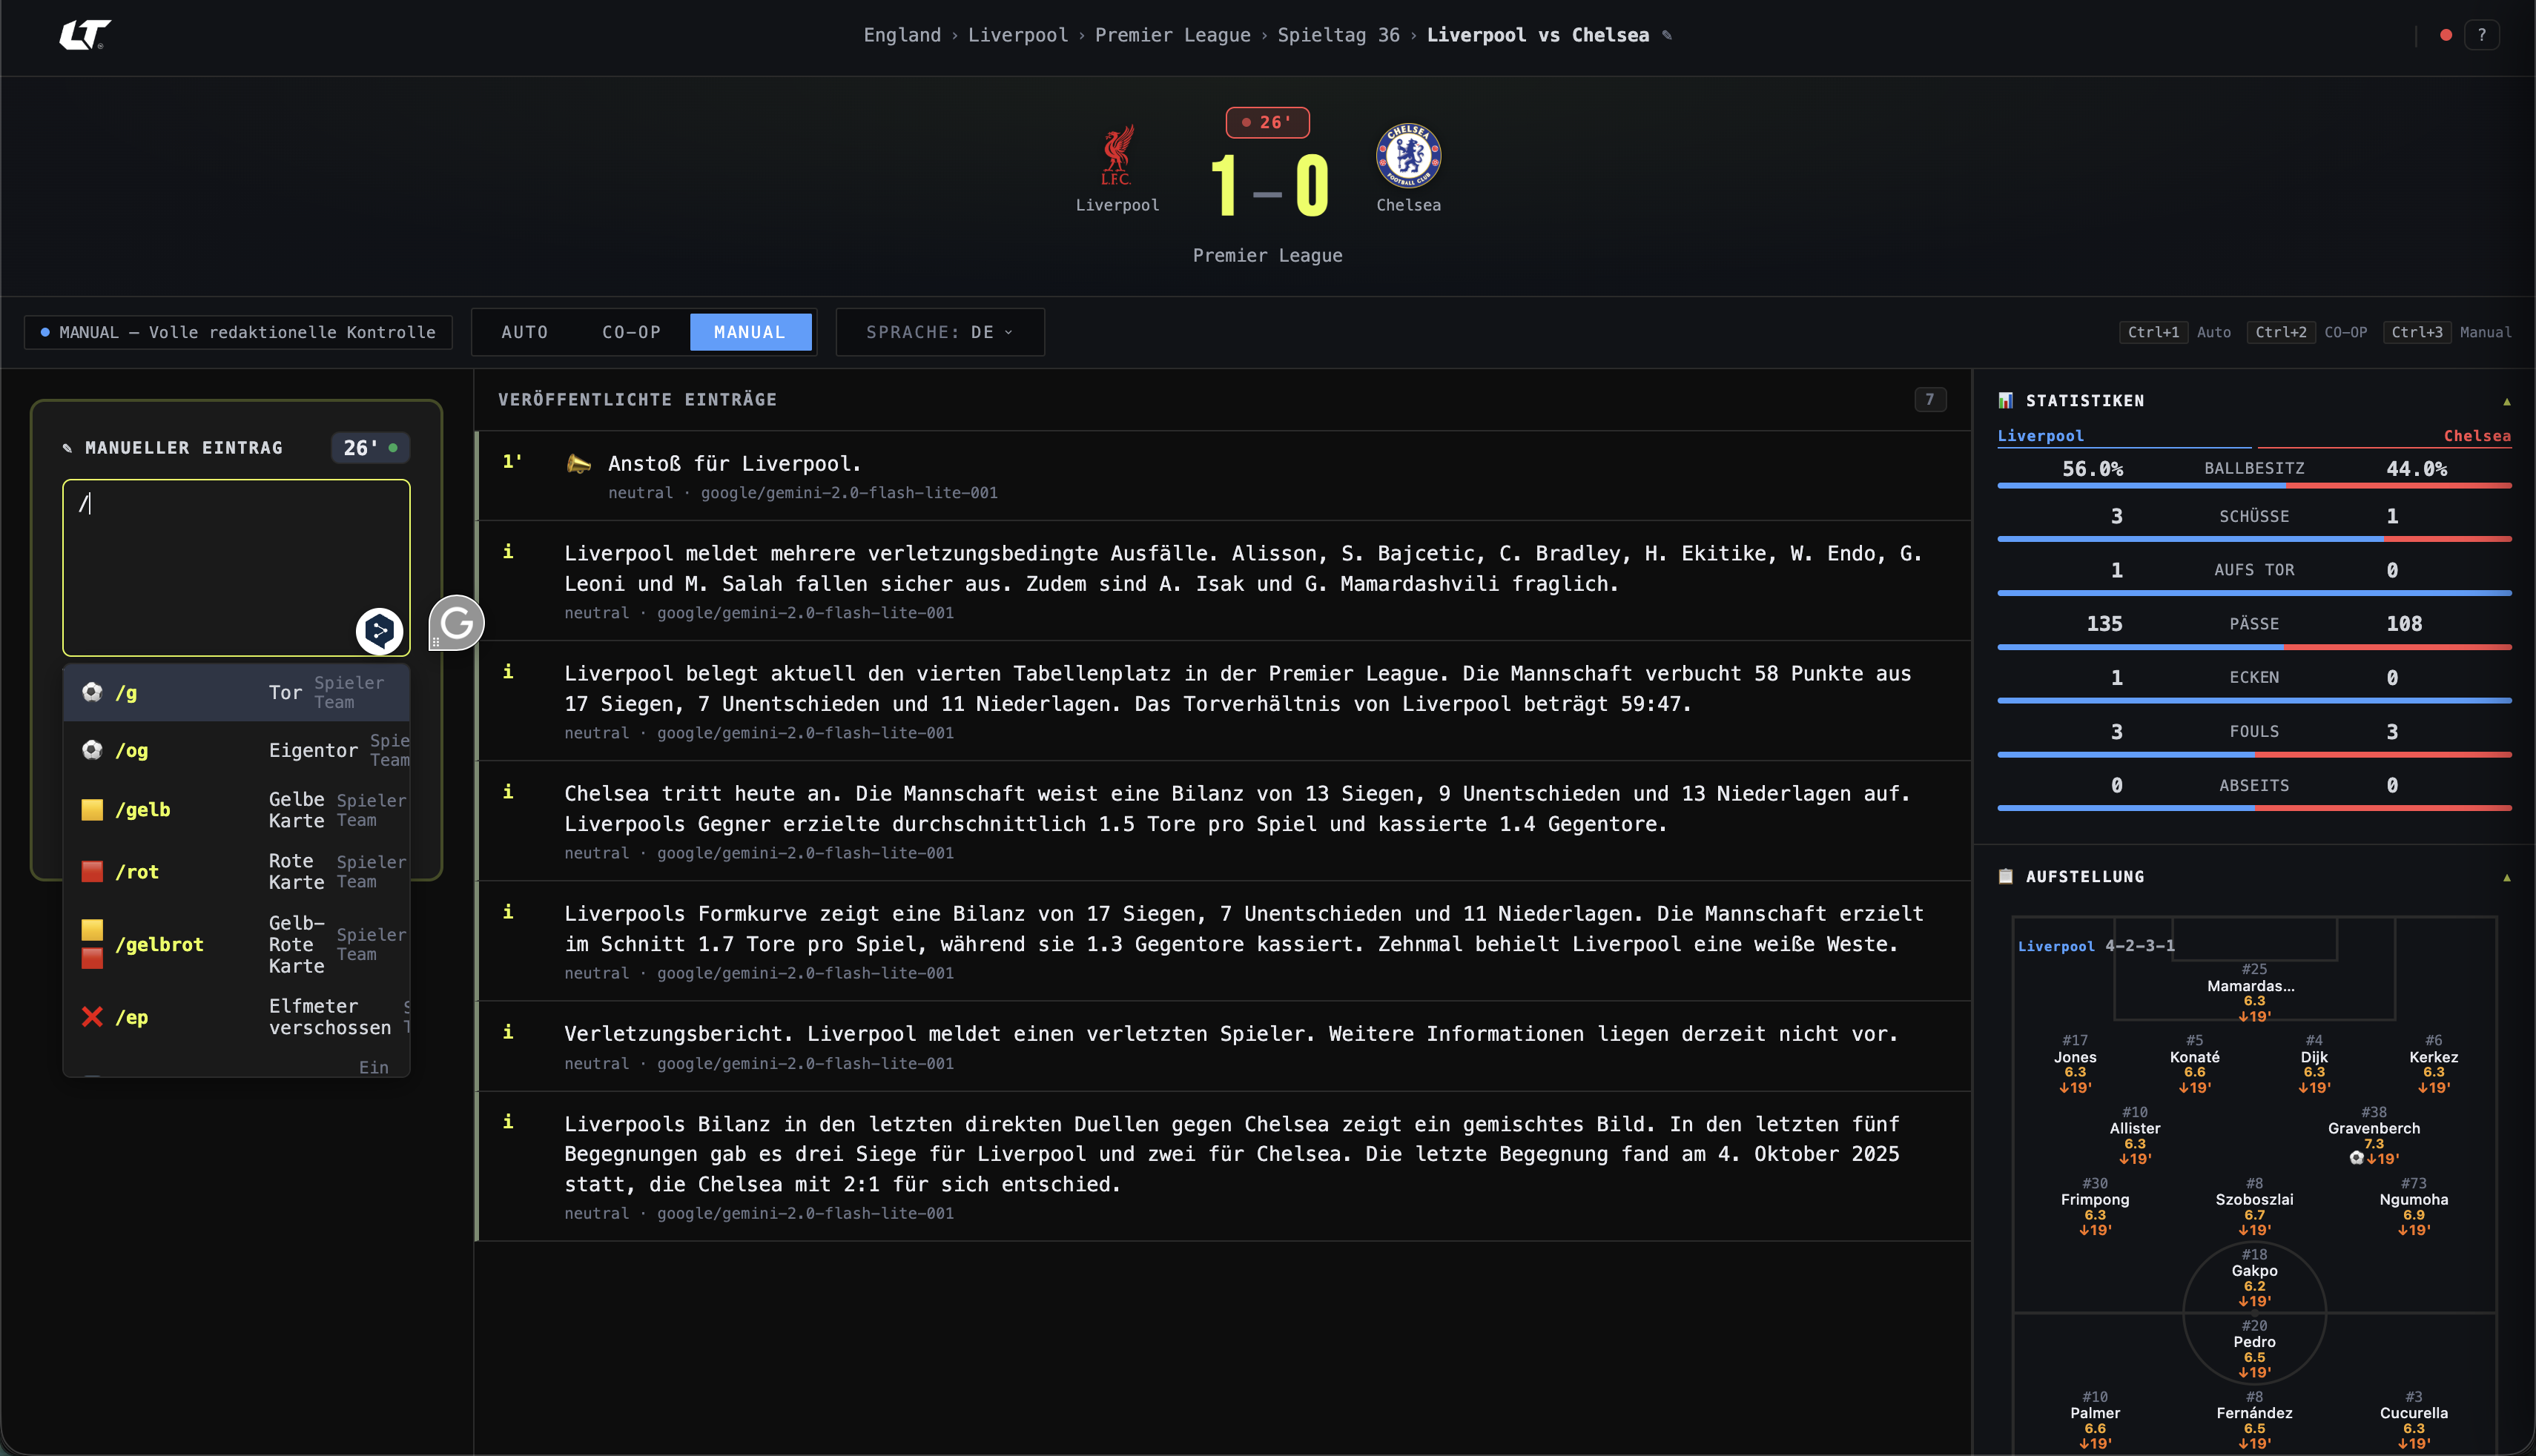
\includegraphics[width=\textwidth]{frontend_slash_command.png}
\caption[Slash-Command-Parser: Eingabe \texttt{/g Müller SGE}]{Slash-Command-Parser: Eingabe \texttt{/g Müller SGE} erzeugt einen strukturierten Ticker-Eintrag mit Icon, Minute und formatiertem Text ohne Backend-Aufruf.}
\label{fig:frontend-slash-command}
\end{figure}


\subsection{Modusimplementierung im
Frontend}\label{modusimplementierung-im-frontend}

Der aktive Modus (\texttt{auto} / \texttt{coop} / \texttt{manual})
steuert das Verhalten mehrerer Frontend-Komponenten (vgl. Abschnitt~\ref{dreispalten-layout-und-redaktionsfluss}).
\texttt{useTickerMode} initialisiert den Modus lokal mit \texttt{coop}
als Standardwert, überschreibt diesen beim Laden eines Spiels mit dem in
der Datenbank gespeicherten \texttt{ticker\_mode} und schreibt
Änderungen per \texttt{PATCH\ /matches/\{id\}/ticker-mode} sofort ans
Backend zurück. Optimistic-Updates vermeiden wahrnehmbare Latenz beim
Umschalten. Die Shortcuts \texttt{Ctrl+1} / \texttt{Ctrl+2} / \texttt{Ctrl+3} für die Modusumschaltung sind in der \texttt{ModeSelector}-Komponente als globaler \texttt{keydown}-Listener registriert. \texttt{useTickerMode} registriert zusätzlich \texttt{TAB} (acceptDraft) und \texttt{ESC} (rejectDraft) als Keyboard-Event-Listener, die nur im Co-op-Modus aktiv sind und bei Moduswechsel automatisch aktualisiert werden.

Im Auto-Modus existieren zwei parallele Automatisierungspfade: Der primäre Pfad verläuft über n8n, das \texttt{auto\_publish=True} an den Backend-Endpunkt übergibt, woraufhin der Eintrag direkt mit \texttt{status=published} angelegt wird. Der sekundäre Pfad ist \texttt{useAutoPublisher} im Frontend: Dieser Hook pollt die Draft-Queue und publiziert neu eintreffende Entwürfe unmittelbar, als Fallback für verzögerte n8n-Webhooks oder bei direkter Modusumschaltung im Frontend ohne n8n-Neustart. Die Deduplizierungsprüfung per \texttt{event\_id} verhindert Doppelveröffentlichungen auf beiden Pfaden.

\begin{figure}[H]
\centering
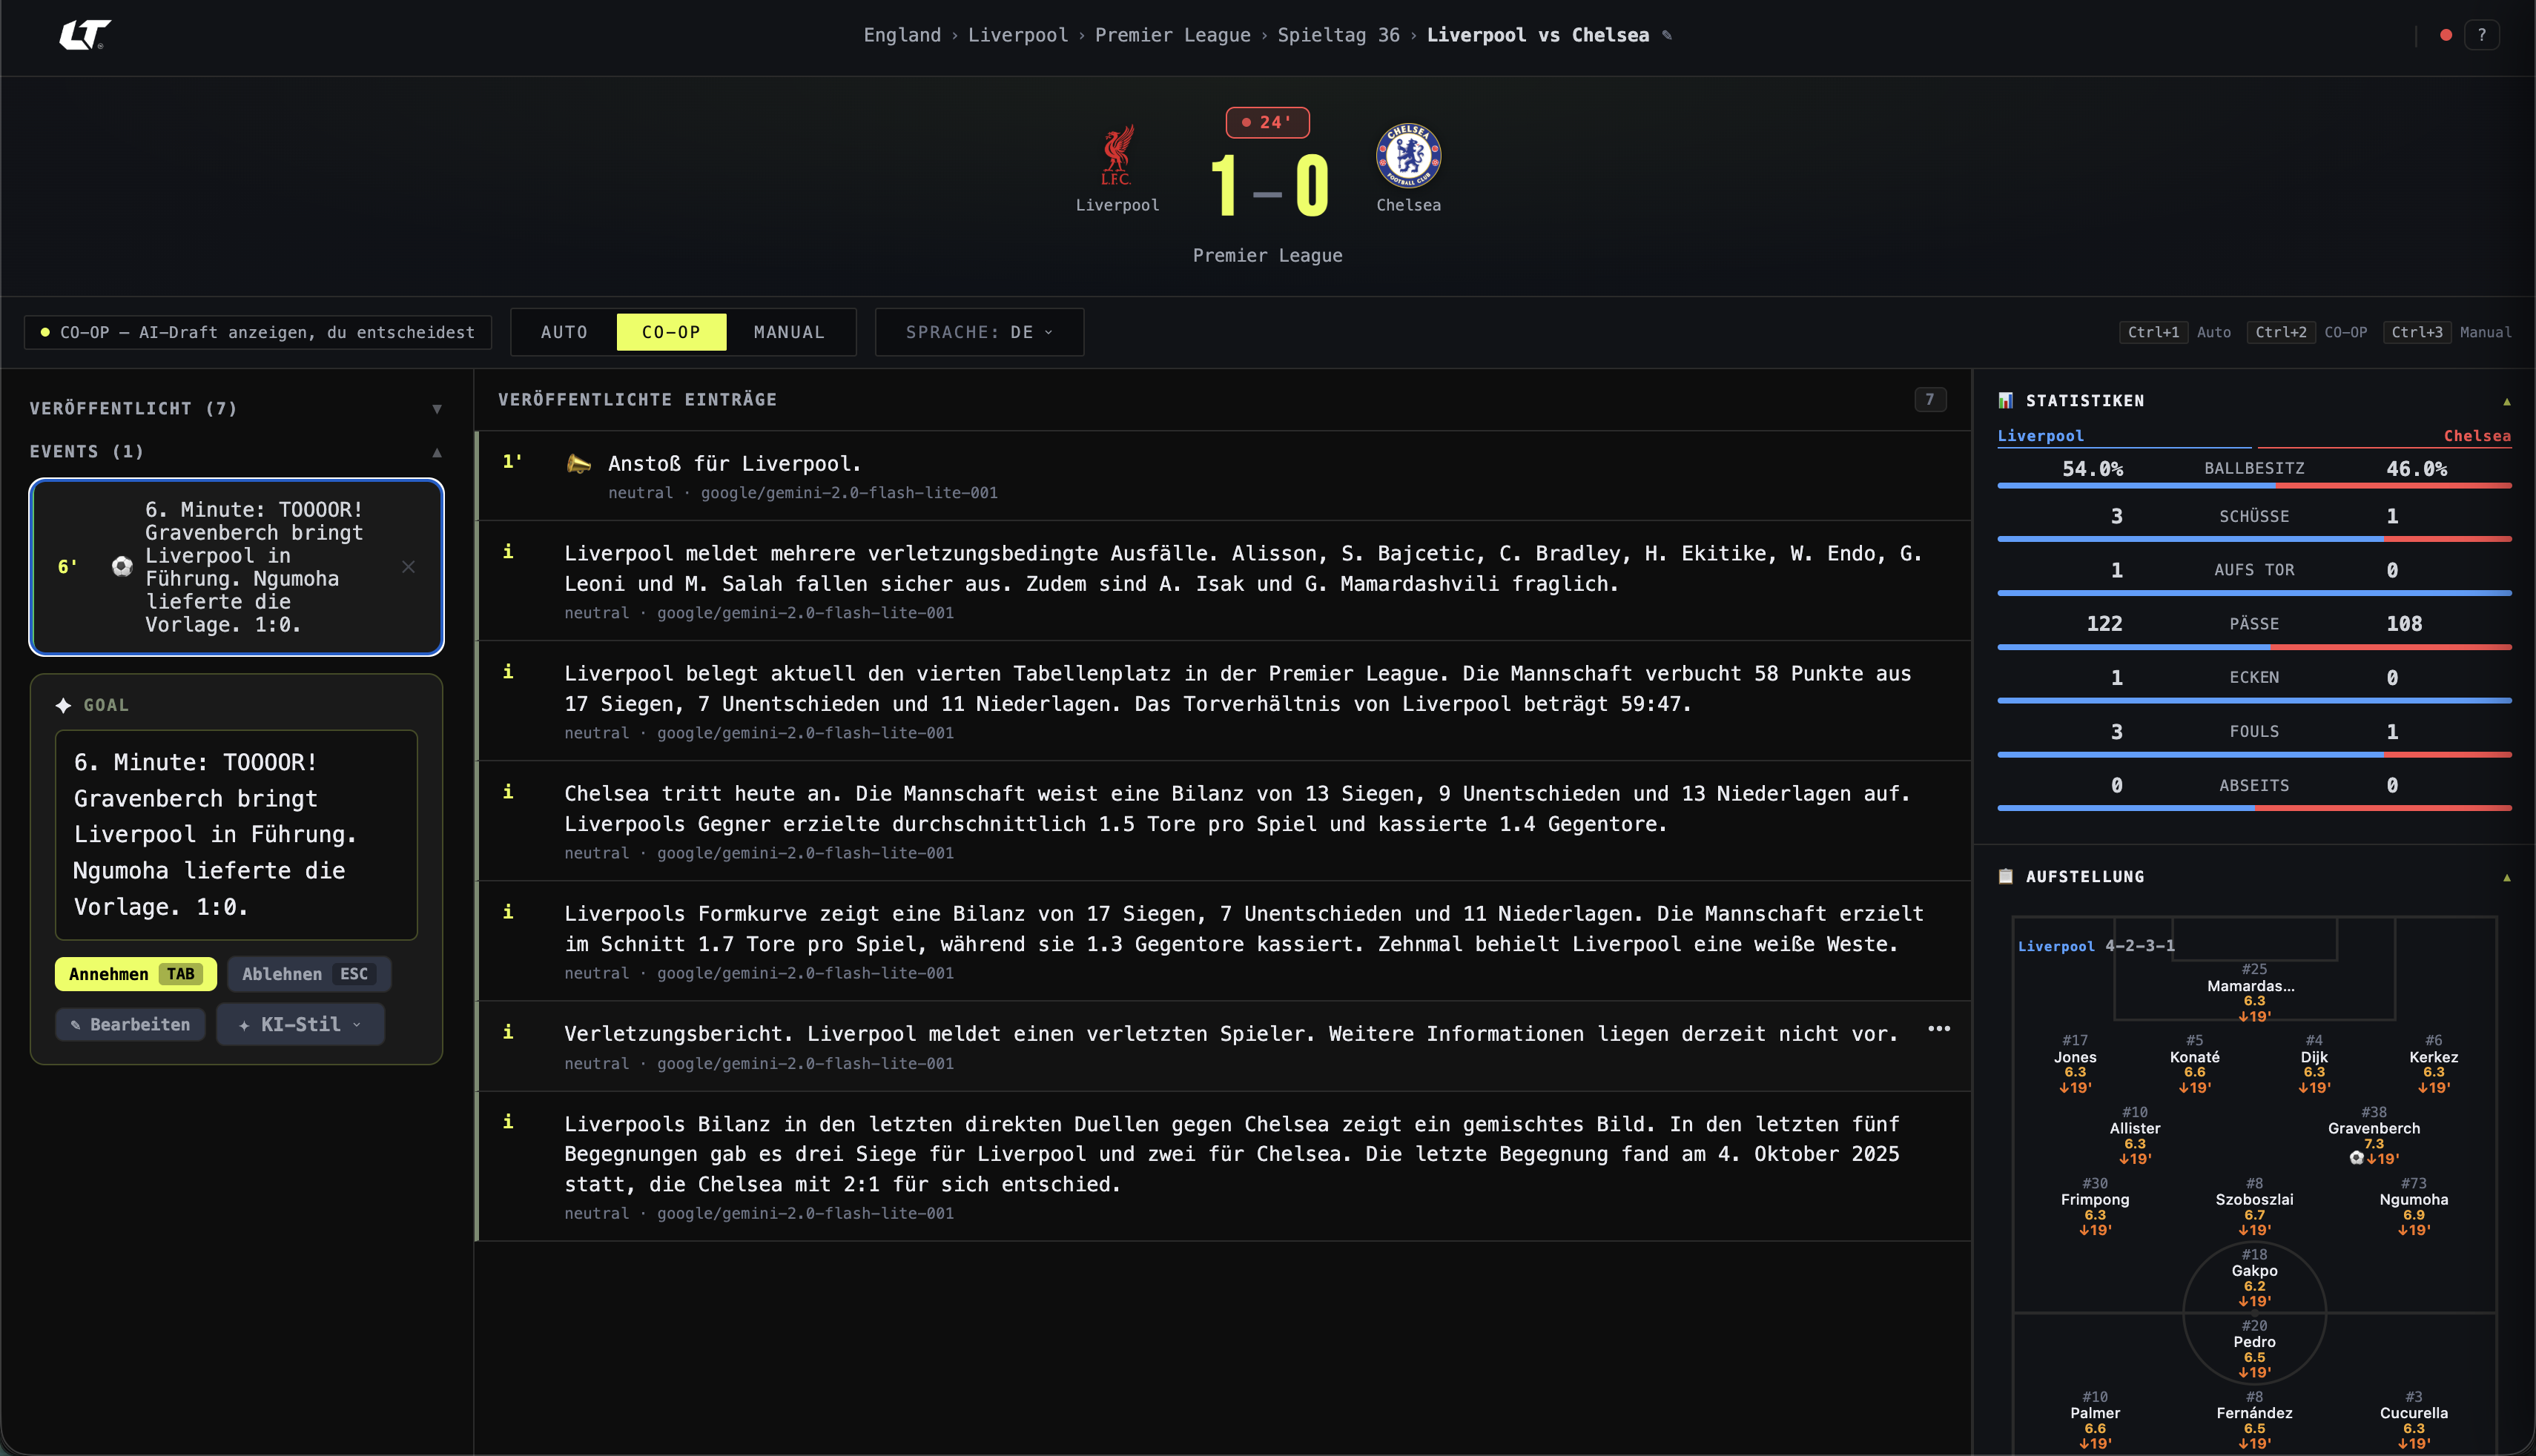
\includegraphics[width=\textwidth]{frontend_coop.png}
\caption[LiveTicker-Editor im Coop-Modus]{LiveTicker-Editor im Coop-Modus: Links KI-generierte Entwürfe (Freigabe per TAB, Ablehnung per ESC), Mitte publizierte Ticker-Einträge, Rechts Spielstatistiken und Kontext. Bei Eintracht-Spielen (\texttt{ef\_whitelabel}) erscheinen links zusätzlich vier Media-Panels unterhalb der Draft-Queue: ein ScorePlay-Bilder-Panel (\texttt{MediaPickerPanel}) sowie YouTube-, Twitter/X- und Instagram-Panels. Das ScorePlay-Panel zeigt Torjubel-Videos und Bilder des Torschützen, die per Doppelklick direkt als Ticker-Eintrag veröffentlicht werden können.}
\label{fig:frontend-coop}
\end{figure}

Der Übergang \texttt{published~→~draft} (Undo) ist im Frontend als Toast-Aktion realisiert: Nach jeder Publikation erscheint für 5~Sekunden ein Widerruf-Button. Über \texttt{PATCH /api/v1/ticker/\{id\}} mit \texttt{\{"status": "draft"\}} wird der Eintrag zurückgesetzt und steht erneut zur Bearbeitung bereit.

Für publizierte Ticker-Einträge bietet das Frontend zwei weitere Eingriffsmöglichkeiten, die unabhängig vom Toast-Fenster verfügbar sind: Jeder Eintrag in der Publikationsliste (LeftPanel) trägt ein Drei-Punkte-Menü (\texttt{EntryMenu}), das \textit{Bearbeiten} und \textit{Löschen} anbietet. Der Bearbeiten-Pfad öffnet ein Inline-Textarea, dessen Änderung per \texttt{PATCH /api/v1/ticker/\{id\}} persistiert wird. Der Löschen-Pfad zeigt einen Bestätigungsdialog und ruft anschließend \texttt{DELETE /api/v1/ticker/\{id\}} auf, das den Eintrag per Soft-Delete auf \texttt{status=deleted} setzt. Für Spielphasen- und Zusammenfassungs-Einträge existiert ein zweiter Retract-Pfad: Die \texttt{PublishedSummarySection} im CenterPanel zeigt alle publizierten Phasen-Einträge in einem einklappbaren Abschnitt „Veröffentlicht". Jeder Eintrag trägt dort einen \textit{↩~Stornieren}-Button, der \texttt{PATCH /api/v1/ticker/\{id\}} mit \texttt{\{"status": "draft"\}} aufruft und den Eintrag wieder in die Draft-Queue zurückführt.


\subsection{Frontend-Polling}\label{frontend-polling}

Das Frontend fragt den Backend-Status über drei Polling-Ressourcen ab:

{\def\LTcaptype{none} % do not increment counter
\begin{longtable}[]{@{}llp{7cm}@{}}
\toprule\noalign{}
Ressource & Intervall & Bedingung \\
\midrule\noalign{}
\endhead
\bottomrule\noalign{}
\endlastfoot
Events, Ticker, Matchdaten & 15.000\,ms & Live, FullTime, null (Standardwert) \\
Events, Ticker, Matchdaten & 20.000\,ms & PreMatch und alle anderen Zustände \\
Spielminuten-Sync & 60.000\,ms & Live, PreMatch, ToBeConfirmed \\
\end{longtable}
}

Die \texttt{resolvePollingInterval}-Utility differenziert das Intervall je nach Spielstatus: Im Live-Modus, bei Spielende (\texttt{FullTime}) und bei noch nicht geladenem Spielstatus (\texttt{null}) beträgt es 15.000\,ms. In allen anderen Zuständen (PreMatch, Pause u.\,a.) gilt 20.000\,ms. Davon getrennt ist \texttt{useLiveMinute}: Dieser Hook berechnet die angezeigte Spielminute, liest aber primär \texttt{match.minute} aus der Datenbank, der von n8n WF16 bei jedem Spielminuten-Update gesetzt wird. Nur wenn \texttt{match.minute} null ist, berechnet \texttt{useLiveMinute} die Minute lokal aus der Anstoßzeit und aktualisiert diese Berechnung alle 30\,s.


\section{n8n Workflow-Implementierung}\label{n8n-workflow-implementierung}

Die n8n-Implementierung realisiert die 17 Workflows als versionierte JSON-Exporte unter \texttt{n8n/}. Durchgängiges Implementierungsziel ist Idempotenz: Jeder Workflow muss wiederholbar auslösbar sein, ohne Dateninkonsistenzen oder redundante LLM-Generierungen zu verursachen. Sie gliedert sich in einen Workflow-Überblick (Abschnitt~\ref{workflow-ueberblick}), die Spielzeit-Kette (Abschnitt~\ref{spielzeit-kette}), den Events-LLM-Workflow (Abschnitt~\ref{events-llm-workflow}) sowie übergreifende Implementierungsmuster (Abschnitt~\ref{n8n-implementierungsmuster}).

\subsection{Workflow-Überblick}\label{workflow-ueberblick}

\begin{figure}[H]
\centering
\DiagramWorkflowTimeline
\caption{Zeitliche Aktivität der n8n-Workflows über einen Spieltag}
\label{fig:workflow-timeline}
\end{figure}

Abbildung~\ref{fig:workflow-timeline} zeigt die zeitliche Aktivität der Kernworkflows über einen Spieltag. WF07 (Prematch-Import) läuft einmalig vor Spielbeginn und baut den Vorberichtskontext aus fünf parallelen Football-API-Abfragen auf. Die Ergebnisse werden als \texttt{synthetic\_events} mit idempotenter \texttt{ON CONFLICT (match\_id, type) DO UPDATE}-Strategie persistiert. WF16 (Spielminuten-Update) und WF09 (Events-LLM) laufen während beider Halbzeiten kontinuierlich. WF14 (Matchphasen) wird bei jedem Phasenübergang einmalig ausgelöst. WF13 (Zusammenfassungen) wird von WF14 nur bei Halbzeit- und Vollzeit-Übergängen nachgelagert getriggert. WF15 (Live-Stats-Monitor) vergleicht aktuelle Football-API-Statistiken per JavaScript-Knoten gegen bereits publizierte Ticker-Einträge und löst nur bei inhaltlich neuen Fakten einen direkten OpenRouter-Aufruf aus. WF08 (ScorePlay-Medien) sucht bei Torereignissen nach Bild-Assets des Torschützen, normalisiert dabei Umlaute im Namen und gleicht ihn gegen vier ScorePlay-Namensfelder ab. Gefundene Asset-URLs überträgt WF08 an \texttt{POST /api/v1/media/incoming} im FastAPI-Backend, das sie über den WebSocket-Kanal (\texttt{/ws/media}) in Echtzeit an das Frontend-Media-Panel weiterleitet. WF10--12 importieren Social-Media-Inhalte aus X, YouTube und Instagram idempotent in die \texttt{media\_clips}-Tabelle. WF01--06 stellen den initialen Datenbasis-Import sicher. Diese beiden Gruppen sind nicht phasengebunden und im Diagramm nicht dargestellt.

\subsection{Spielzeit-Kette}\label{spielzeit-kette}

WF16 (Spielminuten-Update) fragt bei jedem Aufruf die Football-API nach aktuellem Spielstand und Spielphase und vergleicht das Ergebnis mit dem Datenbankstand. Erkennt er eine Phasenänderung, aktualisiert er Spielminute und Phase in der Datenbank und triggert WF14 (Matchphasen-Workflow) über einen internen Webhook-Aufruf.

WF14 validiert den Übergang gegen eine JavaScript-seitige Zustandsmatrix erlaubter Vorzustände, um inkonsistente Wechsel abzufangen. Jeder Übergang erzeugt genau ein synthetisches Event für die neue Phase (z.\,B. \texttt{match\_kickoff} bei Anpfiff, \texttt{match\_fulltime} bei Abpfiff) und aktualisiert den Spielzustand in der Datenbank. Eine \texttt{demote}-CTE setzt bereits publizierte Phasen-Texte bei Re-Triggern auf \texttt{draft} zurück, sodass Korrekturen jederzeit möglich bleiben.

Am Ende eines WF14-Durchlaufs triggert ein HTTP-Request-Knoten WF13 (Zusammenfassung) — jedoch nur bei Halbzeit- (\texttt{HT}) und Vollzeit-Übergängen (\texttt{FT}), da ausschließlich diese Phasen eine redaktionelle Zusammenfassung erfordern. WF13 lädt sequenziell über vier HTTP-Request-Knoten Spieldaten (Backend-API), Spielereignisse, Teamstatistiken und Spieler-Ratings (Football-API) und bettet sie in einen umfangreicheren Prompt ein. Da das Datenvolumen die Eingabelimits des generischen Backend-Endpunkts überschreiten würde, ruft WF13 OpenRouter für den LLM-Aufruf direkt auf, ohne den FastAPI-LLM-Service einzubinden. Das generierte Ergebnis wird anschließend über \texttt{POST /api/v1/ticker/manual} im Backend persistiert, wobei \texttt{ticker\_mode} den initialen Status (\texttt{published} oder \texttt{draft}) bestimmt.

\subsection{Events-LLM-Workflow}\label{events-llm-workflow}

\begin{figure}[H]
\centering
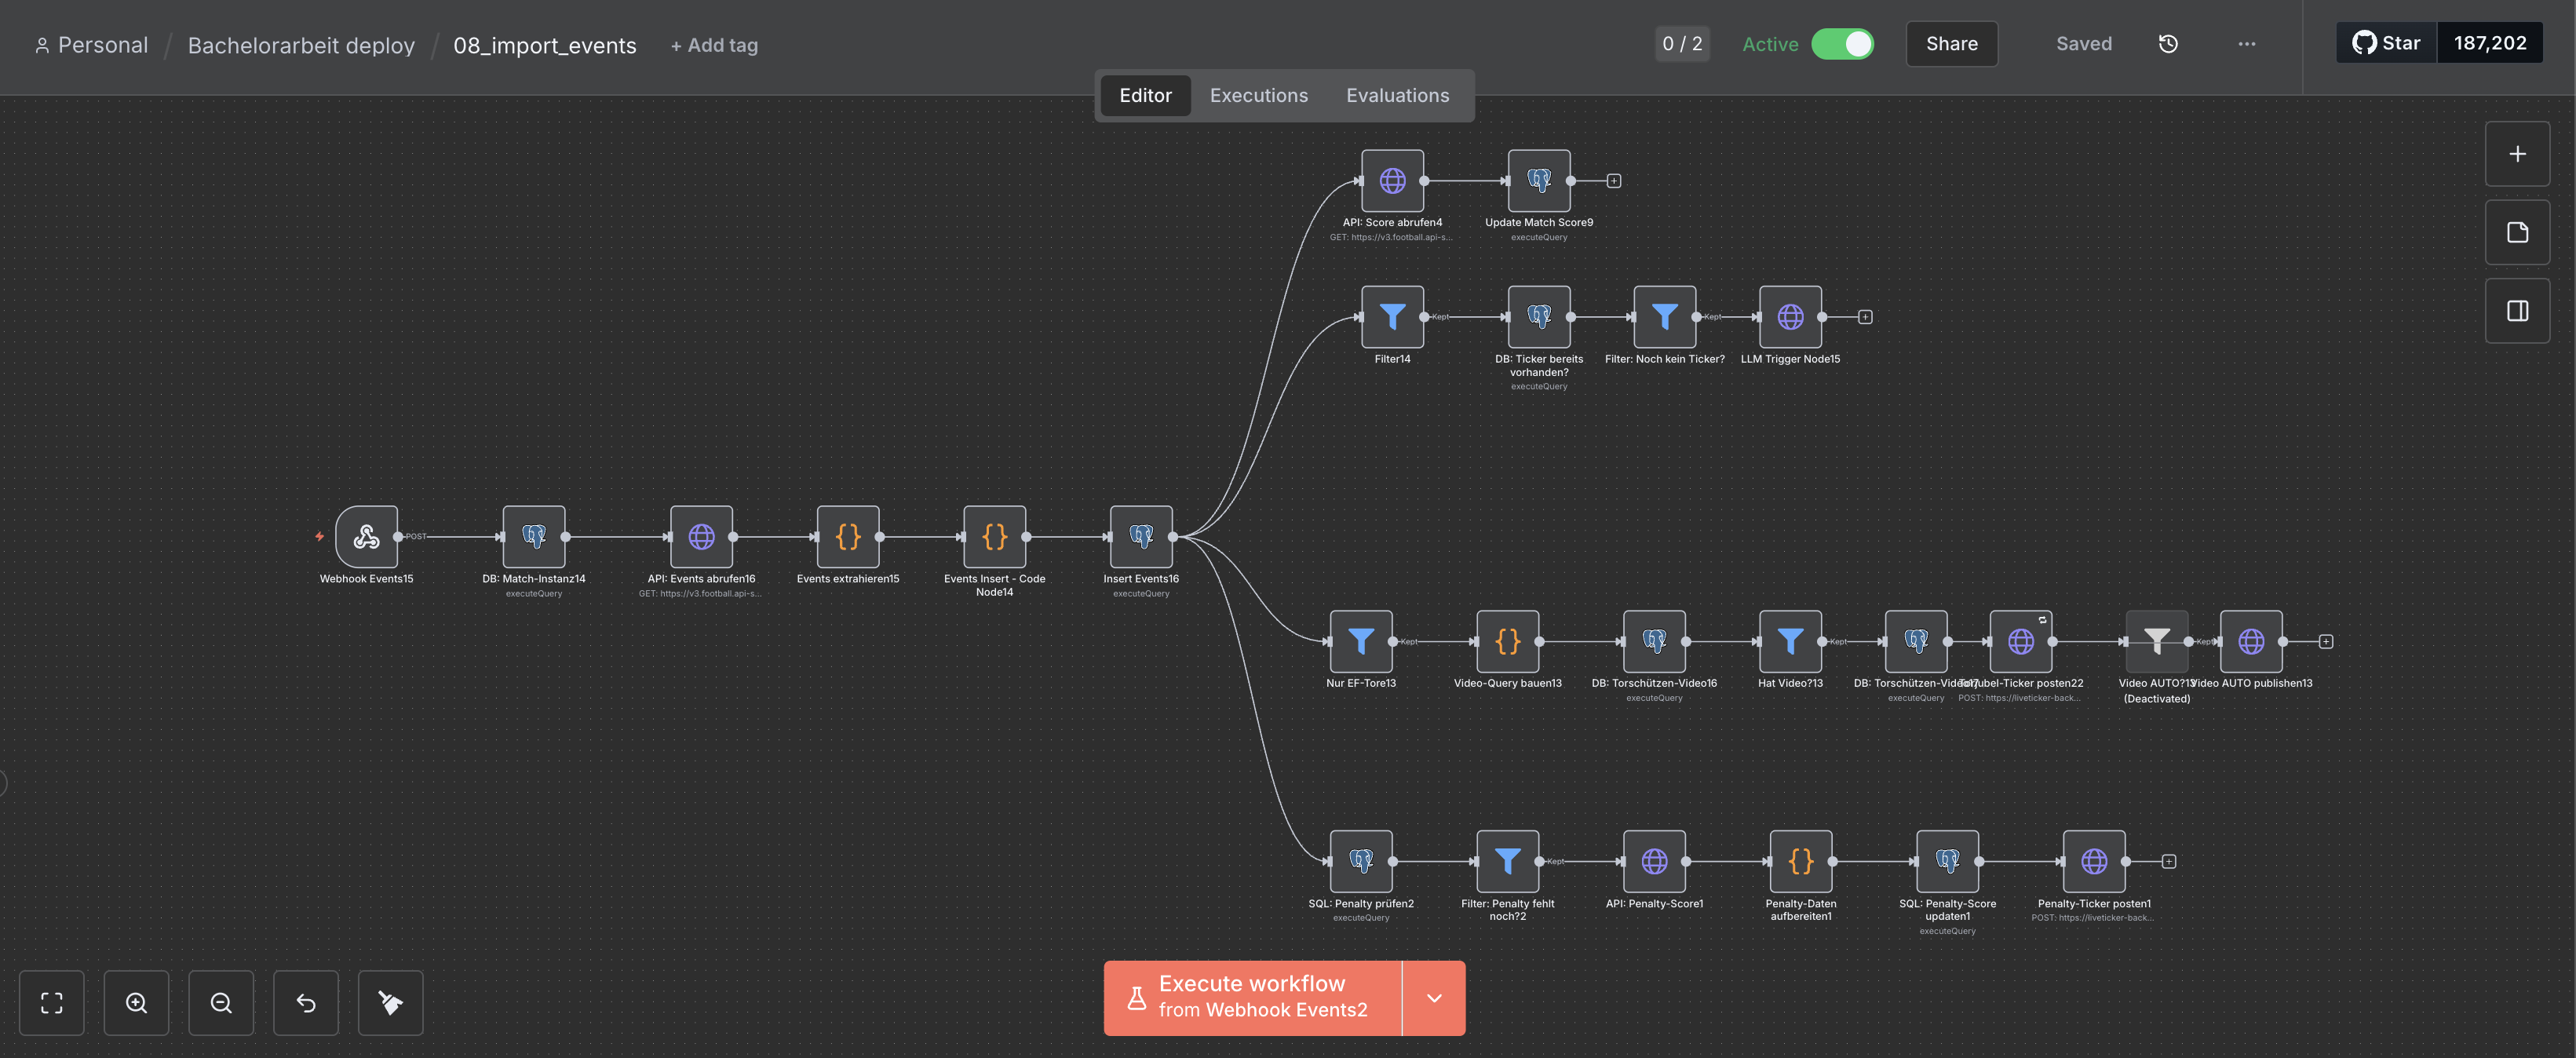
\includegraphics[width=\textwidth]{n8n_event_workflow.png}
\caption[Events-LLM-Workflow (09): Ablauf und Instanz-Routing]{Events-LLM-Workflow (09): Webhook-Eingang, UPSERT in PostgreSQL, Instanz-Routing (\texttt{ef\_whitelabel} / \texttt{generic}), LLM-Trigger und EF-spezifischer Video-Zweig.}
\label{fig:n8n-event-workflow}
\end{figure}

WF09 ist der kritischste Workflow im System. Er wird via Webhook (\texttt{POST /Events}) ausgelöst, der \texttt{fixture\_id} und Zielsprache trägt, und ruft anschließend die Football-API ab, um aktuelle Spielereignisse zu laden und per UPSERT (\texttt{ON CONFLICT (source\_id) DO UPDATE SET}) idempotent zu persistieren. Eine initiale SQL-Abfrage bestimmt anhand der Teamzugehörigkeit (\texttt{ILIKE '\%Frankfurt\%'}) Instanz (\texttt{ef\_whitelabel} oder \texttt{generic}) und Stilprofil des Spiels. \texttt{auto\_publish} wird als \texttt{ticker\_mode === 'auto'} ausgewertet und direkt an den Generate-Endpunkt übergeben. Nur Events mit erfolgreicher Datenbankzeile passieren den Filter-Knoten. Vor dem LLM-Trigger prüft ein eigener DB-Query, ob für das Event bereits ein Ticker-Eintrag existiert. Dieser Workflow-seitige Dedup-Schutz ergänzt den Backend-seitigen Dedup aus Abschnitt~\ref{pipeline-mechanik-und-idempotenz} und verhindert redundante LLM-Aufrufe bei WF09-Wiederholungsläufen. Bei Torereignissen aktualisiert WF09 zusätzlich \texttt{home\_score} und \texttt{away\_score} in der \texttt{matches}-Tabelle über einen separaten Football-API-Aufruf. Ein EF-spezifischer Zweig sucht per SQL-Abfrage in der \texttt{players}-Tabelle nach einer hinterlegten \texttt{video\_url} des Torschützen und persistiert den Video-Link als separaten Ticker-Eintrag (Icon~\texttt{🎬}). Das Instanz-Routing in WF09 setzt die White-Label-Konzeption aus Abschnitt~\ref{partner-team-konzept-und-white-label-steuerung} auf Workflow-Ebene um.

\subsection{Übergreifende Implementierungsmuster}\label{n8n-implementierungsmuster}

Die n8n-Implementierung folgt vier konsistenten Implementierungsentscheidungen, die sich durch die Analyse der Workflow-JSON-Exporte identifizieren lassen:

\begin{itemize}\tightlist
\item \textbf{UPSERT-Strategien:} Alle Insert-Operationen verwenden \texttt{ON CONFLICT DO UPDATE} oder \texttt{DO NOTHING}, um Idempotenz bei Mehrfachausführung sicherzustellen.
\item \textbf{Filter-Knoten:} Vor LLM-Triggern steht jeweils ein Filterknoten, der eine Datenbankzeile nur dann durchlässt, wenn sie eine gültige \texttt{id} enthält \emph{und} als Neu-Insert markiert ist (\texttt{is\_new~=~true}). UPSERT-aktualisierte Events — Ereignisse, die bei einem Wiederholungslauf bereits in der Datenbank lagen — passieren den Filter nicht und lösen keinen redundanten LLM-Aufruf aus.
\item \textbf{Ereignis-Dedup:} WF09 prüft vor dem LLM-Trigger per SQL-Query, ob für das jeweilige Event bereits ein Ticker-Eintrag existiert (\texttt{cnt = 0}-Bedingung). Andere Workflows delegieren diese Prüfung an den Backend-Endpunkt, der bestehende Einträge über \texttt{get\_by\_event()} erkennt und einen Doppeleintrag auf Serviceebene verhindert.
\item \textbf{Mode-Propagation:} \texttt{ticker\_mode} wird als \texttt{auto\_publish}-Flag an das Backend weitergegeben und bestimmt den Publikationsstatus des erzeugten Eintrags.
\end{itemize}


\section{Qualitätssicherung und
Tests}\label{qualituxe4tssicherung-und-tests}

Die Implementierung setzt das in Abschnitt~\ref{qualitätssicherungskonzept} beschriebene Testpyramiden-Modell mit drei Schichten um. Anders als in der Konzeption, wo Teststrategien schichtspezifisch in der Backend- (Abschnitt~\ref{qualitätssicherungskonzept}) und Frontend-Konzeption (Abschnitt~\ref{frontend-teststrategie}) beschrieben sind, werden alle Testebenen hier zusammengefasst, da End-to-End-Tests beide Schichten übergreifen und keiner einzelnen zugeordnet werden können. Sie gliedert sich in Frontend-Tests (Abschnitt~\ref{impl-frontend-tests}), Backend-Tests (Abschnitt~\ref{impl-backend-tests}) und End-to-End-Tests (Abschnitt~\ref{impl-e2e-tests}).

\subsection{Frontend-Tests (Jest + React Testing Library)}\label{impl-frontend-tests}

Unit-Tests decken Utility-Funktionen, Hooks und UI-Komponenten ab. Sieben Hook-Tests sichern das Zustandsmanagement isoliert von der UI ab, darunter \texttt{useMatchEvents}, \texttt{useMatchTicker} und \texttt{useLiveMinute}. Fünf Komponenten-Tests prüfen kritische UI-Elemente: \texttt{EntryEditor}, \texttt{PublishedEntry}, \texttt{CommandPalette}, \texttt{RightPanelComponents} und \texttt{ErrorBoundary}. Der \texttt{parseCommand}-Parser ist mit 45 Testfällen besonders umfangreich abgesichert: Als kritische manuelle Eingabeschicht muss er sämtliche Slash-Command-Varianten, Fehleingaben und Kantenfälle zuverlässig verarbeiten. Ein Fehler hier würde sich direkt in falsch klassierten Ticker-Einträgen niederschlagen. Die folgende Übersicht zeigt die Verteilung auf alle 15 Testdateien.

{\small\def\LTcaptype{none}
\begin{longtable}[]{@{}llr@{}}
\toprule\noalign{}
Datei & Kategorie & Tests \\
\midrule\noalign{}
\endhead
\bottomrule\noalign{}
\endlastfoot
\texttt{useClickOutside.test.ts} & Hook & 5 \\
\texttt{useListKeyboard.test.tsx} & Hook & 9 \\
\texttt{useMatchEvents.test.ts} & Hook & 6 \\
\texttt{useMatchTicker.test.ts} & Hook & 5 \\
\texttt{useLiveMinute.test.ts} & Hook & 10 \\
\texttt{useRightPanelData.test.ts} & Hook & 10 \\
\texttt{useSearchableDropdown.test.ts} & Hook & 10 \\
\texttt{resolvePollingInterval.test.ts} & Utility & 6 \\
\texttt{roundLabel.test.ts} & Utility & 16 \\
\texttt{parseCommand.test.ts} & Utility (Parser) & 45 \\
\texttt{ErrorBoundary.test.tsx} & Komponente & 4 \\
\texttt{CommandPalette.test.ts} & Komponente & 7 \\
\texttt{EntryEditor.test.tsx} & Komponente & 19 \\
\texttt{PublishedEntry.test.tsx} & Komponente & 17 \\
\texttt{RightPanelComponents.test.tsx} & Komponente & 18 \\
\midrule\noalign{}
\textbf{Gesamt} & & \textbf{187} \\
\end{longtable}
}

\subsection{Backend-Tests (pytest)}\label{impl-backend-tests}

API-Integrationstests prüfen die Kern-Endpunkte gegen eine echte PostgreSQL-Testinstanz. Das \texttt{conftest.py}-Setup stellt über ein session-scoped \texttt{reset\_schema}-Fixture (\texttt{drop\_all + create\_all}) einen sauberen Tabellenzustand zu Beginn der Test-Session sicher. Jeder Test erhält eine eigene SQLAlchemy-Session. Nicht committete Änderungen werden nach dem Test zurückgerollt. Committete Stammdaten aus Fixtures bleiben innerhalb der Session erhalten. Repository-Integrationstests und Service-Unit-Tests ergänzen die Abdeckung auf Schichtebene (vgl. Abschnitt~\ref{qualitätssicherungskonzept}): Repository-Tests greifen über die \texttt{db}-Fixture auf die echte Testdatenbank zu. Service-Tests prüfen reine Domänenfunktionen (\texttt{score\_at\_event}, \texttt{build\_match\_context}, \texttt{make\_ai\_entry}) ohne Datenbankabhängigkeit. Der LLM-Service wird in Tests mit \texttt{provider="mock"} instanziiert, da externe LLM-Aufrufe nicht deterministisch und in automatisierten Läufen nicht reproduzierbar sind. Ergänzend enthält \texttt{evaluation\_metrics.py} statistische Hilfsfunktionen (Cliff's Delta, Bootstrap-Konfidenzintervall, Cohen's Kappa u.\,a.) als Evaluationsinfrastruktur für die KI-Textbewertung in Kapitel~\ref{evaluation}. Die folgende Übersicht zeigt die Coverage-Verteilung nach Architekturschicht (246 Tests, 3.230 Statements gesamt).

{\small\def\LTcaptype{none}
\begin{longtable}[]{@{}lr@{}}
\toprule\noalign{}
Schicht & Coverage \\
\midrule\noalign{}
\endhead
\bottomrule\noalign{}
\endlastfoot
Datenmodelle (ORM) & 100\,\% \\
Pydantic-Schemas & 98\,\% \\
Hilfsfunktionen (\texttt{utils}) & 97\,\% \\
Konfiguration (\texttt{core}) & 86\,\% \\
Repositories & 66\,\% \\
Services & 62\,\% \\
API-Router & 59\,\% \\
\midrule\noalign{}
\textbf{Gesamt} & \textbf{79\,\%} \\
\end{longtable}
}

Die unterdurchschnittliche Coverage in API-Router (59\,\%) und Services (62\,\%) ist strukturell bedingt: Endpunkte für externe Medien-Integrationen (\texttt{clips}, \texttt{media}) und die vollständige LLM-Generierungspipeline (\texttt{ticker\_generate}) benötigen externe Dienste, die in automatisierten Läufen nicht reproduzierbar sind. Die Kernfunktionalität (CRUD-Operationen auf Ticker-Einträgen und Spielmetadaten) ist durch die Integrationstests vollständig abgedeckt.

\subsection{End-to-End-Tests (Playwright)}\label{impl-e2e-tests}

Browser-seitige Smoke-Tests in \texttt{e2e/liveticker.spec.ts} validieren grundlegende Nutzerinteraktionen: App-Laden ohne JavaScript-Fehler, Sichtbarkeit des Länder-Dropdowns, Öffnen und Schließen des Keyboard-Shortcuts-Modals über den \texttt{?}-Button sowie ein Viewport-Test bei 375\,×\,812\,px (iPhone~X\,/\,XS\,/\,12\,mini u.\,a.) als Regressionsschutz gegen Layout-Brüche auf kleinen Bildschirmen (N5).

Die vollständige Testsuite umfasst \textbf{187 Frontend-Unit-Tests} in 15 Dateien, \textbf{246 Backend-Tests} in 14 Dateien bei 79\,\% Gesamt-Coverage sowie sechs Playwright-Smoke-Tests. Das Frontend wurde schrittweise auf TypeScript migriert und erreicht im Endstand eine \texttt{type-coverage} von \textbf{98{,}02\,\%} bei null Compilerfehlern (18\,665 von 19\,041 Ausdrücken explizit getypt).


\section{Deployment}\label{deployment}

Das Deployment setzt das in Abschnitt~\ref{deployment-konzept} beschriebene Konzept als produktiv erreichbare Infrastruktur um. Backend und Frontend werden deklarativ über \texttt{render.yaml} im Repository-Branch \texttt{deploy/render-v2} konfiguriert. Datenbank und n8n-Instanz sind externe bzw. lokale Dienste und nicht in \texttt{render.yaml} enthalten.

Das \textbf{FastAPI-Backend} läuft als Docker-Container auf Render.com (Free-Tier Web Service, Region Oregon/US West). Die technologische Einordnung von Docker findet sich in Abschnitt~\ref{cloud-deployment}. Das Docker-Image basiert auf \texttt{python:3.12-slim}. Render deployt automatisch bei jedem Push auf den konfigurierten Branch. Konfiguration und Zugangsdaten werden ausschließlich als Umgebungsvariablen injiziert.

Das \textbf{React-Frontend} wird als statische Seite über das Render-CDN ausgeliefert. Der Build-Prozess führt \texttt{npm ci \&\& npm run build} aus und deployt das \texttt{frontend/build/}-Verzeichnis. Alle Anfragen werden per SPA-Rewrite auf \texttt{index.html} umgeleitet.

Die \textbf{PostgreSQL-15-Datenbank} wird als Managed Service über Supabase betrieben. Das Backend bindet sie über eine externe Connection-URL ein. Supabase übernimmt Backups, Patches und Verbindungspooling ohne operativen Aufwand auf Anwendungsseite.

Die \textbf{n8n-Instanz} läuft lokal als Docker-Container und ist über einen \texttt{ngrok}-Tunnel für externe Webhooks erreichbar. Dieses Setup ist auf den Evaluationszeitraum beschränkt. Die Limitationen gegenüber einem skalierten Produktivbetrieb sind in Abschnitt~\ref{technische-einordnung} diskutiert.

Die vier Komponenten bilden die drei Systemschichten aus Abschnitt~\ref{überblick-und-schichtenmodell}: n8n die Datenbeschaffung, Backend und Datenbank die Anwendungs- und Persistenzlogik, das Frontend die Präsentation. Kapitel~\ref{evaluation} dokumentiert die systematische Evaluation des so realisierten Systems.
